\section{Gestione dei dati multimediali}

I file multimediali rappresentano un elemento centrale all’interno di un’applicazione orientata alla condivisione sociale,
contribuendo significativamente all’esperienza utente e all’interazione tra i partecipanti.
La possibilità di acquisire e condividere contenuti visivi, come immagini e video, consente di documentare eventi e attività,
favorendo una memoria collettiva e rafforzando il legame tra gli utenti.
In particolare, l’integrazione di materiale multimediale associato a eventi condivisi permette di preservare una rappresentazione più completa e dettagliata dell’esperienza vissuta,
migliorando l’engagement e la partecipazione all’interno della piattaforma, rappresentando uno dei punti di forza dell’applicazione.\\
\\
Tuttavia, la gestione dei file multimediali introduce complessità operative sia per gli utenti sia per il sistema stesso.
Da un lato, la selezione e l’invio dei contenuti possono rappresentare un onere significativo per l’utente, aumentando l’attrito nell’utilizzo dell’applicazione.
Per ottimizzare il processo e migliorare l’usabilità, è essenziale semplificare al massimo l’interazione richiesta,
automatizzando il recupero dei dati e limitando il ruolo dell’utente alla semplice conferma dei contenuti selezionati.
Questo approccio non solo semplifica l’esperienza d’uso, ma la rende più intuitiva e fruibile,
contribuendo anche a un incremento del tasso di adozione e della frequenza di utilizzo dell’applicazione.\\
\\
Parallelamente, la memorizzazione e il trasferimento di file multimediali pongono sfide significative a livello infrastrutturale,
in quanto tali dati presentano un impatto rilevante sulle risorse computazionali e sulla gestione dello storage.
Il volume elevato di richieste di caricamento e accesso ai file può infatti compromettere le prestazioni del sistema,
introducendo ritardi causati dal traffico di azioni che potrebbero influire negativamente sulle altre operazioni dell’applicazione.
Per garantire un’archiviazione efficiente e scalabile, è quindi necessario implementare una strategia di gestione della memoria
che separi il salvataggio dei file multimediali dal database principale, evitando di sovraccaricare il server applicativo.
Questa soluzione deve inoltre garantire un aggiornamento tempestivo delle informazioni, assicurando la sincronizzazione tra i dati archiviati e le modifiche effettuate dagli utenti.\\
\\
Per affrontare tali problematiche, un primo esame osserverà le modalità di recupero dei file multimediali,
con un focus sulle tecniche di selezione e rilevamento automatico delle immagini, nonché sui vincoli normativi e di sicurezza che ne regolano l’utilizzo.
In un secondo tempo l’analisi si concentrerà invece sulle strategie di salvataggio e gestione dello storage,
analizzando le diverse tipologie di archiviazione disponibili e le soluzioni implementate per garantire scalabilità, efficienza e riduzione dell’impatto sulle prestazioni del sistema.


\clearpage


\subsection{Recupero}

L’aggiunta di immagini a un evento prevede una fase preliminare di recupero, che consente all’utente di selezionare i file multimediali da associare. 
Il sistema offre due modalità principali di acquisizione: la selezione manuale da parte dell’utente, che può scegliere le immagini direttamente dalla memoria del dispositivo, 
e in alternativa, disponibile sui dispositivi mobili, un meccanismo automatizzato, che identifica le foto scattate durante lo svolgimento dell’evento.\\
\\
L’implementazione di questa funzionalità automatica di analisi della galleria per individuare i file multimediali desiderati  richiede l’accesso alla galleria fotografica del dispositivo, 
un’operazione subordinata al consenso esplicito dell’utente. 
Al primo avvio dell’applicazione perciò, il sistema richiede l’autorizzazione per accedere ai file multimediali, unitamente al permesso per la gestione delle notifiche. 
Nel caso in cui l’utente neghi l’accesso, la richiesta verrà riproposta ogni qualvolta il sistema rilevi la necessità di accedere alla galleria per il recupero delle immagini.\\
\\
Al termine di ogni evento, non appena possibile, l’applicazione avvia automaticamente un’analisi della galleria locale, individuando le immagini scattate durante tutta la durata dell’evento. 
Se il sistema rileva la presenza di contenuti pertinenti, ne memorizza temporaneamente i riferimenti in una memoria locale per poi inviare una notifica all’utente, 
informandolo del ritrovamento delle immagini. A questo punto, l’utente ha la possibilità di esaminare le immagini suggerite, escluderne alcune o confermarne l’intero set per il caricamento.\\
\clearpage
\begin{figure}[htb]
    \centering
    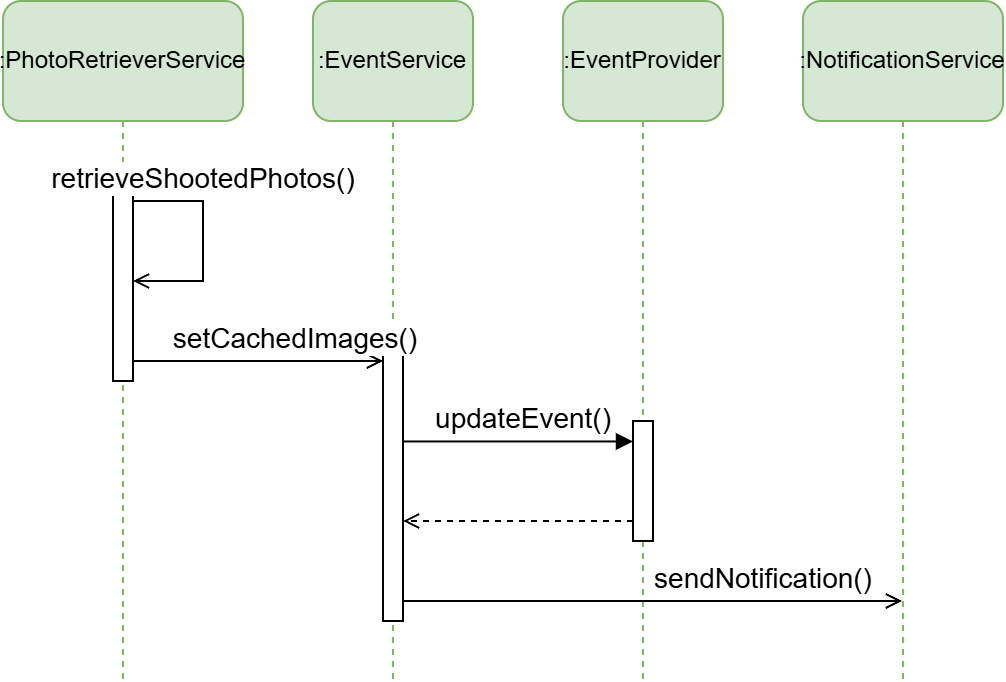
\includegraphics[height=0.45\textheight]{IIRecuperaImmagini.png}
    \caption{Interazione tra i componenti per il recupero delle immagini}
\end{figure}

Questa fase di conferma, oltre a garantire la trasparenza del servizio nei confronti dell’utente, 
riducendo il rischio di errori o caricamenti indesiderati, presenta anche vantaggi in termini di ottimizzazione delle prestazioni. 
\clearpage
Da un punto di vista normativo, la procedura di recupero e selezione automatica delle immagini è esplicitamente descritta nelle condizioni d’uso dell’applicazione, 
alle quali l’utente deve aderire con accettazione espressa prima di utilizzare il servizio. 
Tuttavia, la fase di conferma dell’utente non rappresenta un obbligo giuridico, 
poiché la responsabilità della pubblicazione di contenuti multimediali ricade sul soggetto che realizza la fotografia. 
In conformità con la normativa vigente in materia di tutela dell’immagine (art. 10 c.c. e artt. 96-97 della Legge n. 633/1941) e protezione dei dati personali (Regolamento UE 2016/679 – GDPR), 
chi scatta una fotografia è tenuto a ottenere il consenso delle persone ritratte prima di procedere alla sua pubblicazione.\\
\\
Come già affrontato nel capitolo precedente, le operazioni che coinvolgono la modifica di uno stesso componente del sistema 
sono soggette a vincoli di concorrenza per l’accesso alla risorsa di interesse. 
La conclusione di un evento condiviso tra più utenti potrebbe generare richieste simultanee per l’aggiunta di immagini associate a un medesimo evento. 
L’introduzione della fase di selezione introduce un ritardo nella fase di caricamento, 
dilatando la distribuzione temporale delle richieste e riducendo la probabilità di collisioni dovute a operazioni concorrenti sullo stesso elemento.
L’attesa della conferma dell’utente prevede infatti un ritardo fisiologico tra la fine dell’evento e l’effettivo caricamento delle immagini, 
contribuendo a distribuire le richieste nel tempo e limitando il rischio di congestione del server dovuta a operazioni simultanee su un singolo evento.\\
\\
Una volta completata la selezione da parte dell’utente, le immagini vengono inviate al server, che provvede al loro salvataggio e all’associazione con l’evento corrispondente.


\clearpage

\subsection{Salvataggio}

A differenza dei dati tradizionalmente scambiati all’interno del sistema, i file multimediali presentano dimensioni significativamente superiori, 
con diversità che si manifestano su ordini di grandezza rilevanti. 
Un salvataggio di tali file nel flusso di dati standard, allineandoli agli elementi logici, 
comporterebbe un rallentamento generale delle operazioni e un impatto significativo sulle prestazioni complessive del sistema. 
Per questo motivo, è necessaria una gestione della memoria specificamente progettata per l’archiviazione e il recupero di contenuti multimediali.	\\
\\
Inoltre, Le dimensioni delle immagini e dei video influenzano direttamente il tempo di elaborazione e il volume delle richieste, 
aumentando il carico computazionale su tutti i componenti del sistema. 
In aggiunta, la possibilità di allegare più file a un singolo evento implica che i tempi di caricamento più elevati dei file multimediali 
possano prolungare sensibilmente la durata delle transazioni necessarie per la modifica degli eventi, incidendo sulla reattività del sistema.\\
\\
\clearpage
\subsubsection{Persistenza}

La visualizzazione dei file multimediali riveste un'importanza secondaria rispetto ad altre funzionalità offerte dall'applicazione. 
Di conseguenza, è possibile accettare un maggiore tempo di caricamento, a condizione che ciò contribuisca a ridurre la latenza delle operazioni invece più rilevanti. 
Il salvataggio dei file multimediali direttamente nel database centrale comporterebbe un aumento significativo del volume delle richieste, 
determinando un maggiore impiego di risorse computazionali e un incremento dei tempi di caricamento. 
Questo fenomeno potrebbe incidere negativamente sulle prestazioni complessive del sistema, penalizzando l’esecuzione simultanea di altre operazioni.\\
\\
Per ottimizzare la gestione dei file multimediali, si adotta una distinzione della relazione tra l’oggetto logico e l'evento dai dati binari che lo compongono. 
In questo modo, la relazione tra il file e l’evento associato viene mantenuta indipendentemente dai dati binari che lo compongono. 
Una volta recuperati i riferimenti ai file multimediali associati all’evento in questione, sarà possibile ottenere poi i loro contenuti binari in un secondo momento, solo quando necessario.
Il modello del dominio illustrato in precedenza evidenzia la relazione logica tra gli eventi e i file associati (Photo).\\
\\
Considerando la necessità e la possibilità di archiviare i file multimediali su risorse differenti dal database centrale, 
è fondamentale individuare la soluzione più adatta alla loro persistenza. 
I principali servizi cloud per l’archiviazione di file multimediali si suddividono in tre categorie: Object Storage, File Storage e Block Storage.
Gli Object Storage gestiscono i file in un unico livello, con la possibilità di aggiungere metadati agli oggetti. 
A ciascun elemento viene associato un identificativo univoco che ne consente il recupero. 
L’accesso ai dati avviene tipicamente tramite API RESTful, che oltre ad offrire la possibilità di gestire i permessi, garantisce l’utilizzo su ampia scala. 
La presenza di un unico livello di indirizzamento permette una scalabilità pressoché illimitata, e un costo variabile in base alla quantità di dati memorizzati.
I File Storage organizzano i file in una struttura gerarchica di cartelle e sottocartelle, semplificando la gestione dei file e il controllo degli accessi. 
Oltre a facilitare un controllo ulteriore agli utenti, questa soluzione è compatibile con protocolli di accesso particolari. 
Tuttavia, la sua capacità e scalabilità, così come il costo effettivo, sono legati alla struttura dei file e alla capacità prevista dal piano selezionato.
Infine, i Block Storage gestiscono la memoria tramite la suddivisione dei dati in blocchi logici, salvati separatamente e ognuno dotato di identificativo univoco. 
Questa tecnologia offre elevate prestazioni per il recupero e la modifica dei dati, ma i costi aumentano all'incremento della quantità di dati presenti. 
La scalabilità è quindi limitata alla capacità assegnata al volume. Oltretutto, i costi sono elevati, particolarmente riguardo moli di grandi entità.\\
\\
Tra queste soluzioni, la categoria degli Object Storage risulta la più adatta alle esigenze del progetto di salvataggio dei file multimediali. 
La sua scalabilità illimitata consente di gestire grandi volumi di elementi con una ridotta interdipendenza tra loro. 
Inoltre, l’identificazione univoca di ciascun oggetto garantisce una rapida individuazione dei dati e un’efficiente risposta prestazionale a numerose richieste contemporanee.\\
\\
Nel contesto di Azure, il servizio di Object Storage fornito è rappresentato da Azure Blob Storage (ABS). 
ABS adotta un’organizzazione centrata su Container, entità logiche che raggruppano più file multimediali e introducono un livello di indirizzamento aggiuntivo. 
L’accesso in lettura ai dati avviene tramite protocollo API RESTful, con autenticazione per l’aggiunta di nuovi elementi. 
Per ogni evento viene creato un Container dedicato, contenente le immagini corrispondenti.\\
\\
Terminata la selezione dei file multimediali, prima dell’invio al server, i dispositivi client eseguono la compressione delle immagini, 
riducendo il consumo di banda e il volume dei dati totali trasmessi. 
Questa strategia consente di diminuire il carico computazionale sul server, migliorando l’efficienza complessiva del sistema.\\
\\
Il server, una volta ricevuta la richiesta, esegue una verifica dei permessi di accesso necessari e procede con il caricamento delle immagini nel Container associato all’evento. 
Al termine dell’operazione, il database viene aggiornato con i riferimenti ai nuovi file multimediali, e gli utenti vengono notificati della modifica avvenuta.\\
\\
La visualizzazione di un evento con immagini allegate comporta la richiesta parallela da parte delle singole immagini del dispositivo client verso ABS. 
Le immagini vengono identificate univocamente attraverso la combinazione dell’hash dell’immagine con quello del Container associato all’evento.\\
\\

\begin{figure}[h!]
    \centering
    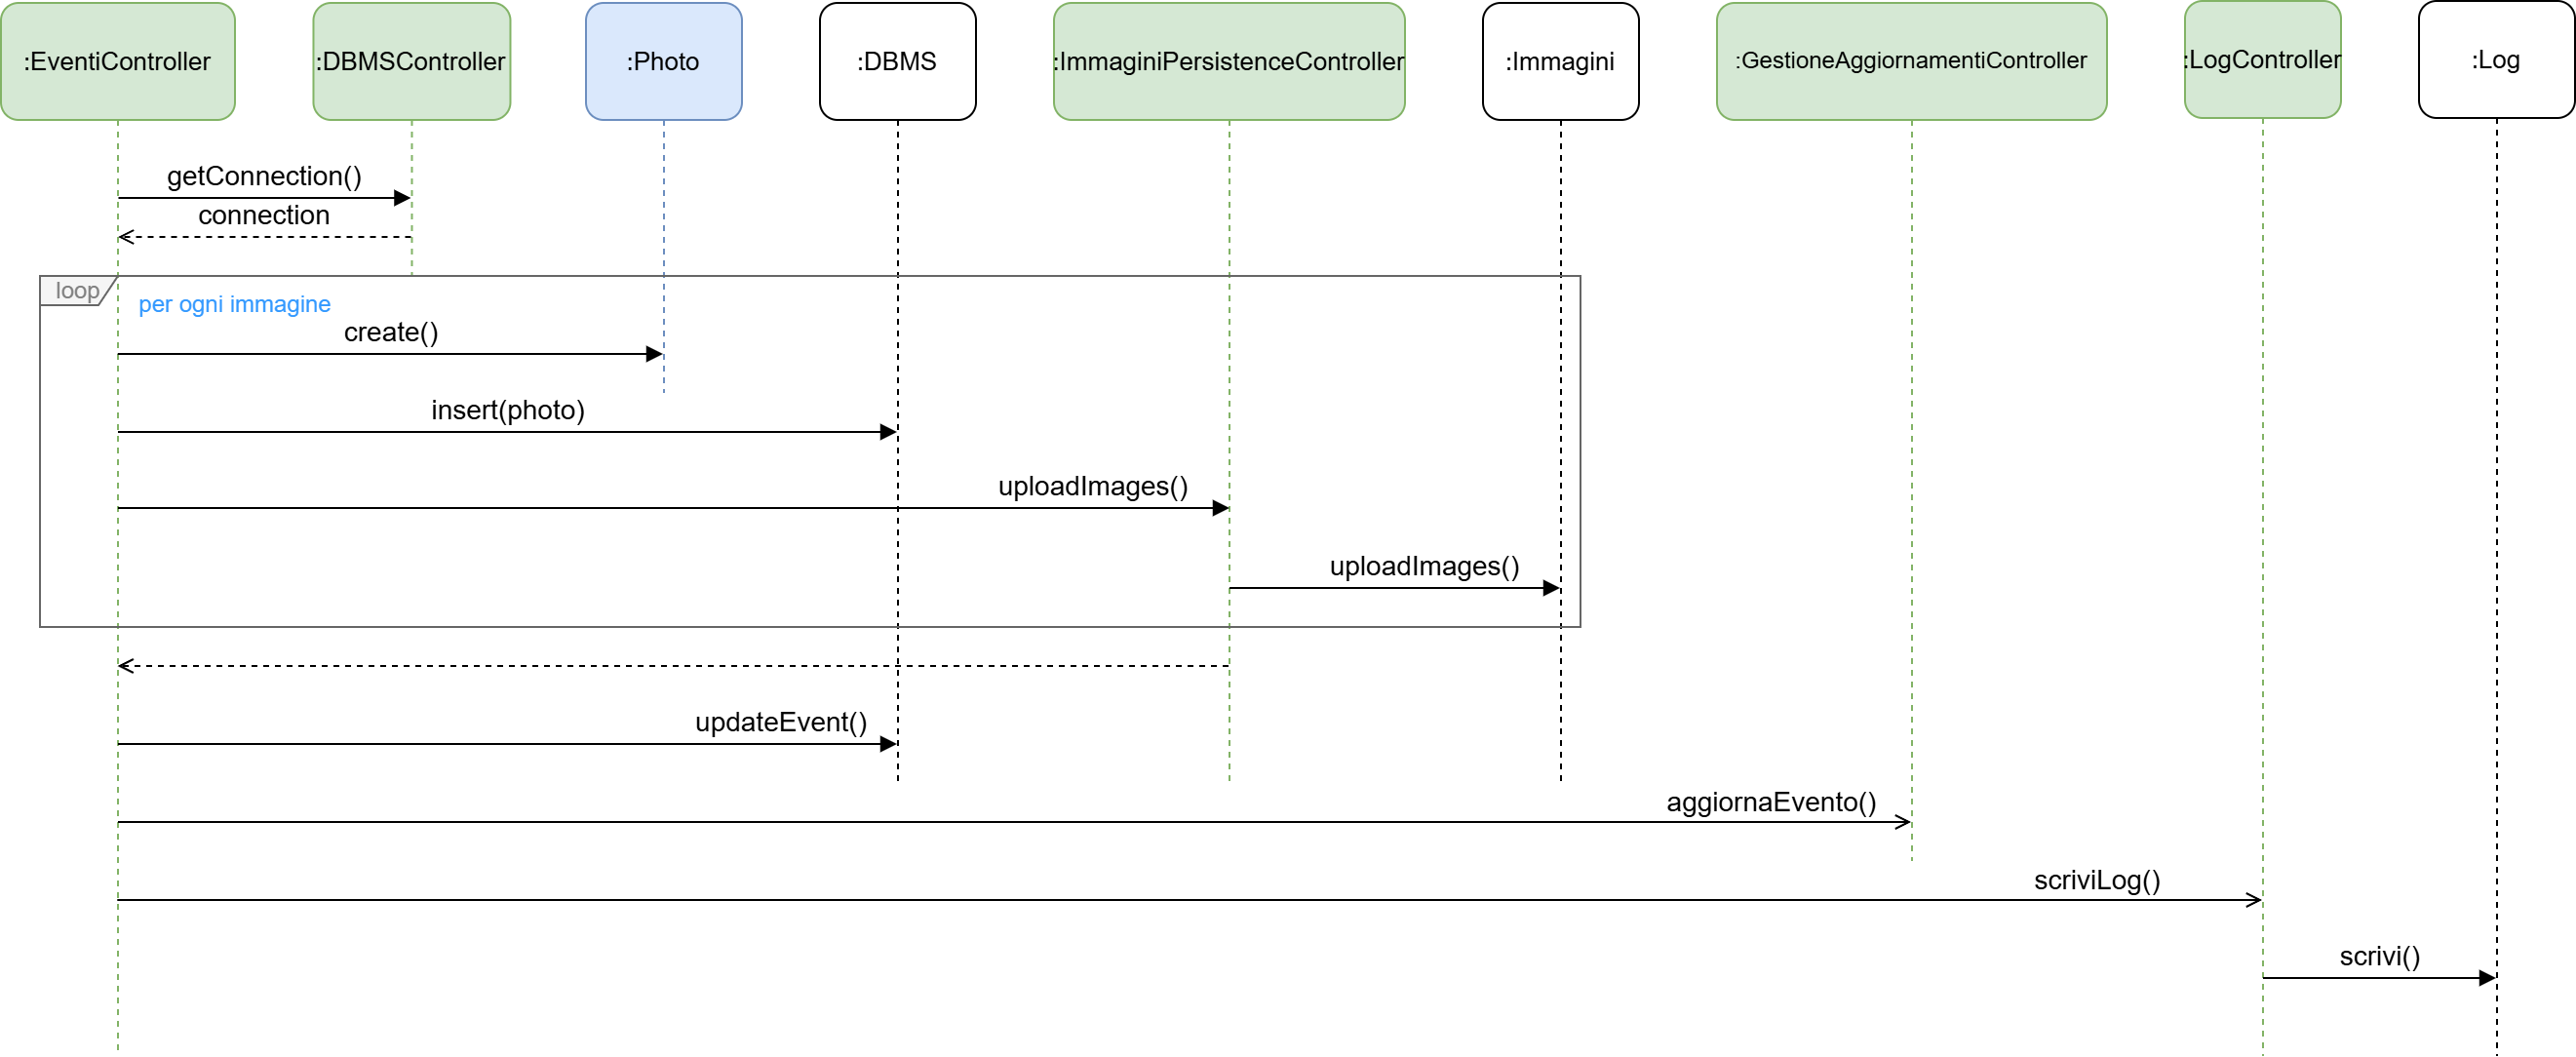
\includegraphics[width=\textwidth]{PIConfermaImmagini2.png}
    \caption{Interazione progettuale del server per il caricamento delle immagini }
\end{figure}

Tuttavia, l’accesso in lettura ai file multimediali in ABS risulta pubblico per impostazione predefinita, 
poiché la mancata definizione di ruoli comporta l’assenza di controlli espliciti sulle autorizzazioni delle richieste. 
Questo aspetto viene mitigato mediante l’uso di hash randomici sufficientemente lunghi, che riducono drasticamente la probabilità di collisione. 
Senza la conoscenza dell’hash corretto, un accesso non autorizzato alle immagini 
richiederebbe tentativi casuali estremamente numerosi nella speranza di trovare una combinazione corretta, rendendo un attacco altamente improbabile. 
Inoltre, anche in caso di compromissione di un hash, l’accesso sarebbe limitato a una singola immagine, senza fornire ulteriori informazioni sugli altri file memorizzati.

\clearpage

\subsubsection{Concorrenza }

Il caricamento delle immagini dalle Azure Functions al Container associato all’evento rappresenta un'operazione relativamente onerosa in termini di tempo, 
soprattutto se confrontata con le altre operazioni eseguite dal sistema. 
La gestione delle connessioni tra il server e il database relazionale richiede dunque scelte di dominio e sviluppo mirate a garantire un uso ottimale delle risorse, 
minimizzando il tempo di blocco e migliorando l'efficienza complessiva.\\
\\
Un elemento centrale nel processo di invio dati è la gestione dell’hash dell’elemento Photo, che deve corrispondere al file caricato. 
L’hash viene generato al momento della creazione dell’oggetto, ma il suo salvataggio nel database avviene solo dopo il completamento del caricamento del file multimediale. 
Questa strategia evita operazioni di scrittura e cancellazione superflue, ottimizzando le prestazioni del sistema. 
Ne consegue che il momento della creazione dell’oggetto Photo deve essere logicamente distinto dal suo effettivo salvataggio nel database.

Per realizzare un’astrazione ad alto livello della relazione con il database, Entity Framework Core (EF Core) fornisce una rappresentazione logica degli elementi, 
mantenendo un collegamento con le relative controparti fisiche. 
Grazie a questa caratteristica, è possibile creare un oggetto senza doverlo immediatamente memorizzare, consentendo un controllo più preciso e immediato sul flusso dei dati.\\
\\
La relazione uno a molti tra gli eventi e le immagini è implementata mappando fisicamente  sugli oggetti Photo, 
i quali contengono un riferimento all’identificativo dell’evento associato. 
Al momento del salvataggio, viene modificata esclusivamente la tabella relativa a Photo; 
tuttavia, tale operazione implica un blocco in scrittura anche sull’oggetto Event. 
Ciò avviene poiché l’oggetto Event è coinvolto a livello logico, come dimostrato anche dalla presenza di una lista virtuale contenente le immagini associate tra i suoi attributi.\\
\\
Per migliorare l’efficienza del caricamento, la trasmissione dei file multimediali verso il Container avviene in parallelo, 
riducendo il tempo complessivo necessario per completare l’operazione. 
Tuttavia, l’inserimento immediato di ciascun oggetto Photo nel database al termine di ogni caricamento comporterebbe un rischio di conflitti sull’oggetto Event 
e un potenziale sovraccarico del database. Per mitigare questi problemi, 
gli oggetti logici Photo delle trasmissioni avvenute con successo vengono temporaneamente conservati in memoria per essere salvati successivamente  in un’unica operazione.\\
\\
L'inserimento simultaneo di tutti gli elementi Photo validi all'interno di una stessa transazione consente di ottimizzare l’impatto sul database, 
riducendo i tempi di blocco sull’oggetto Event e minimizzando il rischio di collisioni tra richieste concorrenti. 
Questo approccio garantisce una maggiore scalabilità e una gestione più efficiente delle risorse del sistema coinvolte.\\
\\

\begin{figure}[h!]
    \centering
    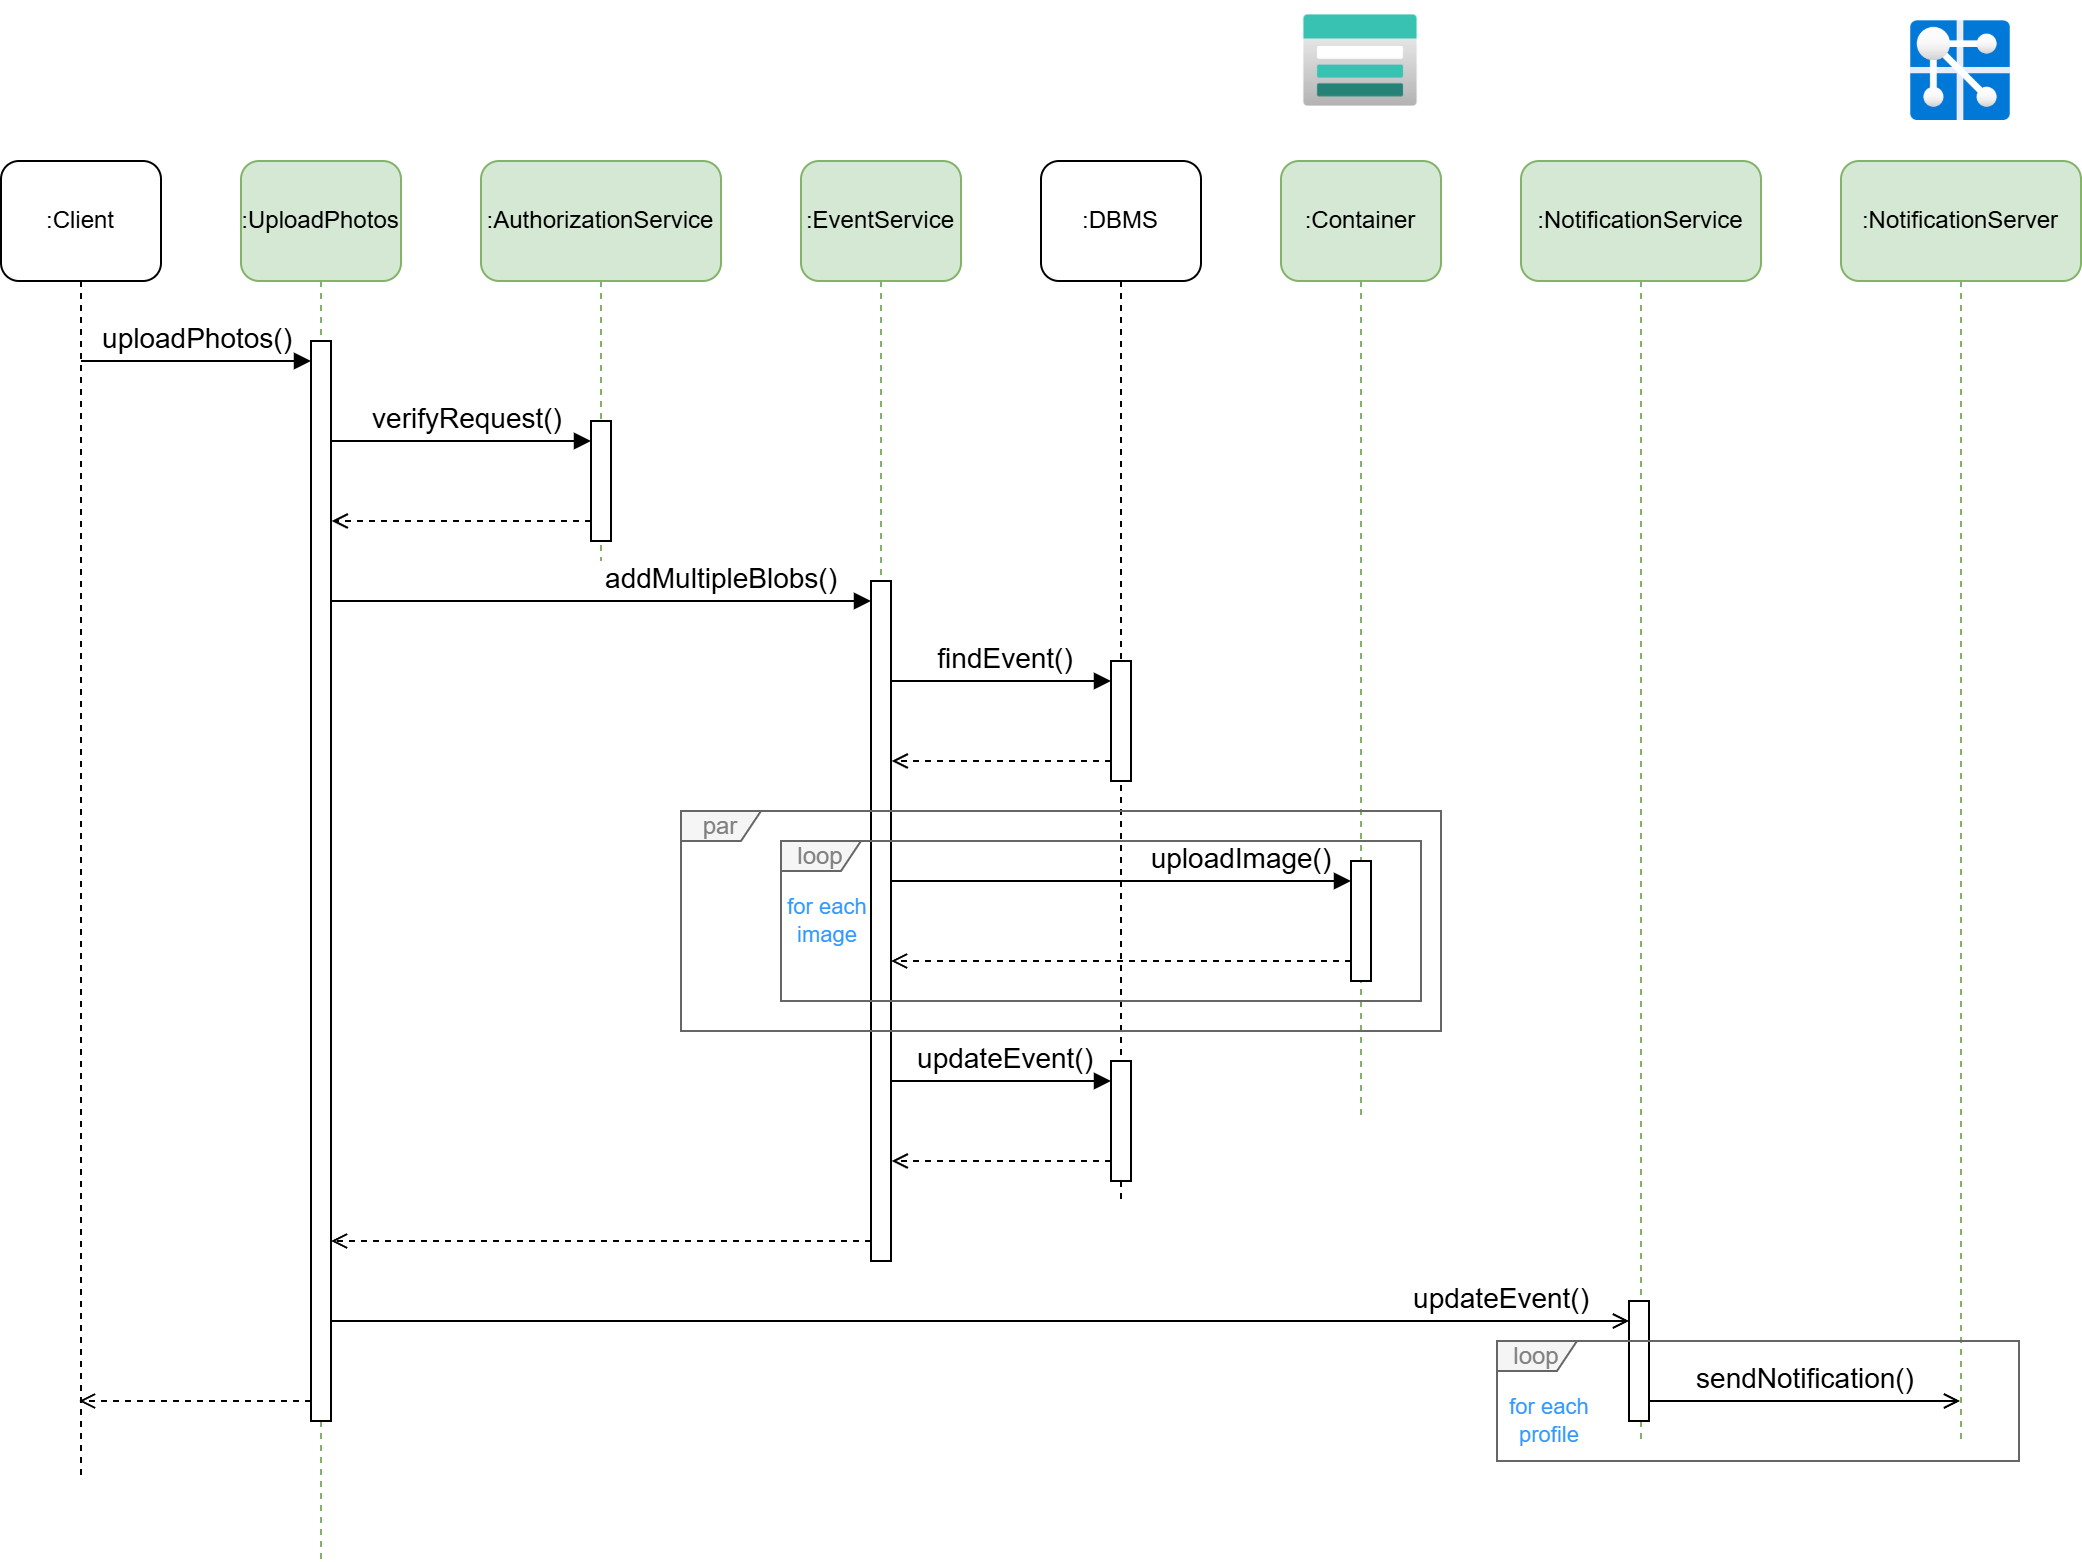
\includegraphics[width=\textwidth]{IICaricaImmagini.png}
    \caption{Interazione logica del server per il caricamento delle immagini }
\end{figure}

\clearpage